\documentclass[12pt,letterpaper,twoside]{article}
\usepackage{cme211}
\usepackage{algorithm2e}

\def\D{\mathrm{d}}
\usepackage{atbegshi}% http://ctan.org/pkg/atbegshi
\AtBeginDocument{\AtBeginShipoutNext{\AtBeginShipoutDiscard}}

\begin{document}
\title{Lecture 15: Boost\vspace{-5ex}}
\date{November 15th, 2018}
\maketitle

{\footnotesize
\paragraph{Topics:} Functions, Command line arguments and
formatting, (file) IO, pre-processor and \texttt{\#include}.
}
\vspace{-3ex}

\hypertarget{cme-211-lecture-14}{%
\section{CME 211: Lecture 14}\label{cme-211-lecture-14}}

Topics:

\begin{itemize}
\tightlist
\item
  Multi-dimensional data
\item
  Boost \texttt{multi\_array}
\end{itemize}

\hypertarget{layout-in-memory-for-vector}{%
\subsection{\texorpdfstring{Layout in memory for
\texttt{vector}}{Layout in memory for vector}}\label{layout-in-memory-for-vector}}

\begin{figure}
\centering
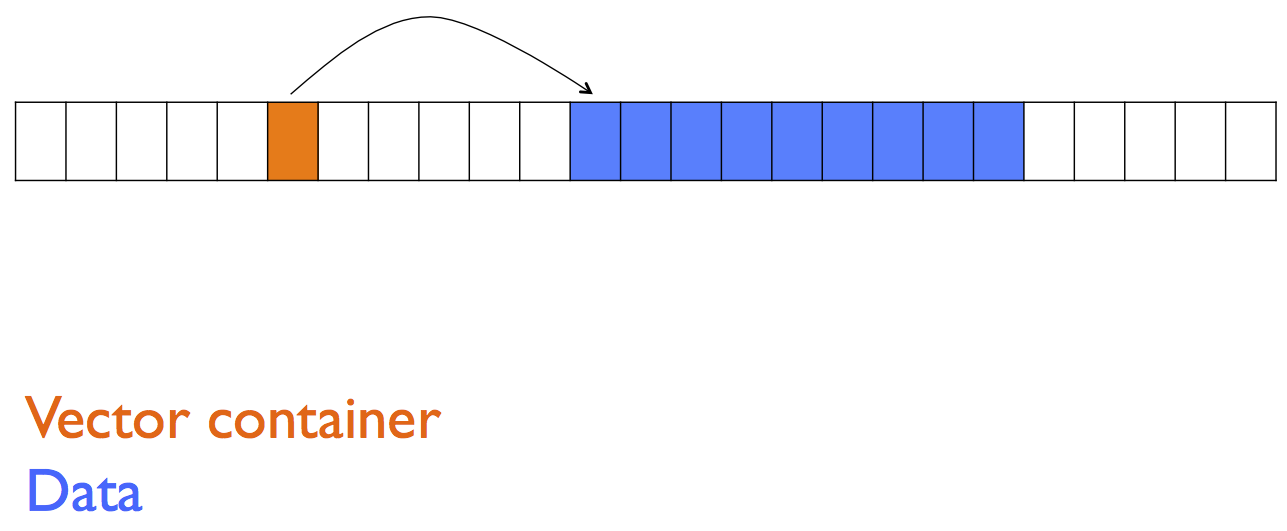
\includegraphics{fig/vector-memory.png}
\caption{fig}
\end{figure}

\begin{itemize}
\item
  Memory for \texttt{std::vector} has 2 parts:

  \begin{itemize}
  \item
    Memory for the vector data
  \item
    Memory for the \texttt{std::vector} container. This part
    (essentially) includes the memory address of the vector data, the
    size of the vector and capacity.
  \end{itemize}
\item
  The 2 parts may be very far apart in the memory address space.
\end{itemize}

\hypertarget{look-at-the-details}{%
\subsubsection{Look at the details}\label{look-at-the-details}}

\texttt{src/vector\_memory.cpp}:

\begin{Shaded}
\begin{Highlighting}[]
\PreprocessorTok{#include }\ImportTok{<iostream>}
\PreprocessorTok{#include }\ImportTok{<vector>}

\DataTypeTok{int}\NormalTok{ main() \{}
  \BuiltInTok{std::}\NormalTok{vector<}\DataTypeTok{int}\NormalTok{> a;}
  \ControlFlowTok{for}\NormalTok{ (}\DataTypeTok{int}\NormalTok{ i = }\DecValTok{0}\NormalTok{; i < }\DecValTok{10}\NormalTok{; i++) \{}
\NormalTok{    a.push_back(i);}
\NormalTok{  \}}
  \BuiltInTok{std::}\NormalTok{cout << }\StringTok{"sizeof(a): "}\NormalTok{ << }\KeywordTok{sizeof}\NormalTok{(a) << }\BuiltInTok{std::}\NormalTok{endl;}
  \BuiltInTok{std::}\NormalTok{cout << }\StringTok{"    memory location of a: "}\NormalTok{ << &a << }\BuiltInTok{std::}\NormalTok{endl;}
  \BuiltInTok{std::}\NormalTok{cout << }\StringTok{" memory location of data: "}\NormalTok{ << a.data() << }\BuiltInTok{std::}\NormalTok{endl;}
  \BuiltInTok{std::}\NormalTok{cout << }\StringTok{"difference in memory loc: "}
\NormalTok{            << }\DataTypeTok{double}\NormalTok{((}\DataTypeTok{int}\NormalTok{*)&a-a.data()) / }\DecValTok{1024}\NormalTok{ / }\DecValTok{1024}\NormalTok{ / }\DecValTok{1024} 
\NormalTok{            << }\StringTok{" GB"}\NormalTok{ << }\BuiltInTok{std::}\NormalTok{endl;}
  \ControlFlowTok{return} \DecValTok{0}\NormalTok{;}
\NormalTok{\}}
\end{Highlighting}
\end{Shaded}

Output:

\begin{verbatim}
$ clang++ -std=c++11 -Wall -Wextra -Wconversion src/vector_memory.cpp -o src/vector_memory
$ ./src/vector_memory
sizeof(a): 24
    memory location of a: 0x7fff57a18870
 memory location of data: 0x7ff6d3403310
difference in memory loc: 8.51711 GB
$ ./src/vector_memory
sizeof(a): 24
    memory location of a: 0x7fff56bd4870
 memory location of data: 0x7f8c5ac03310
difference in memory loc: 114.984 GB
$ ./src/vector_memory
sizeof(a): 24
    memory location of a: 0x7fff52c5e870
 memory location of data: 0x7fb08bd00040
difference in memory loc: 78.7772 GB
\end{verbatim}

\begin{itemize}
\item
  The size of the \texttt{std::vector} container is 24 bytes, this could
  be for

  \begin{itemize}
  \item
    8 bytes for the memory address of the vector data
  \item
    8 bytes for the size of the vector, number of elements stored
  \item
    8 bytes of the capacity of the vector, number of elements that may
    be stored before reallocation
  \end{itemize}
\item
  Memory locations are different in each run of the program. This is a
  security feature to make it harder to introduce malicious code or
  data.
\end{itemize}

\hypertarget{multidimensional-data}{%
\subsection{Multidimensional data}\label{multidimensional-data}}

\begin{itemize}
\tightlist
\item
  How do we handle multidimensional data in C++?
\end{itemize}

\hypertarget{container-of-containers}{%
\subsubsection{Container of containers}\label{container-of-containers}}

\texttt{src/multi1.cpp}:

\begin{Shaded}
\begin{Highlighting}[]
\PreprocessorTok{#include }\ImportTok{<vector>}
\PreprocessorTok{#include }\ImportTok{<iostream>}

\DataTypeTok{int}\NormalTok{ main() \{}
  \CommentTok{// declare vector of vectors}
  \BuiltInTok{std::}\NormalTok{vector< }\BuiltInTok{std::}\NormalTok{vector<}\DataTypeTok{double}\NormalTok{> > v;}
  \CommentTok{// add empty "second-level" vectors}
\NormalTok{  v.push_back(}\BuiltInTok{std::}\NormalTok{vector<}\DataTypeTok{double}\NormalTok{>());}
\NormalTok{  v.push_back(}\BuiltInTok{std::}\NormalTok{vector<}\DataTypeTok{double}\NormalTok{>());}
\NormalTok{  v.push_back(}\BuiltInTok{std::}\NormalTok{vector<}\DataTypeTok{double}\NormalTok{>());}
  \CommentTok{// add some data}
  \DataTypeTok{double}\NormalTok{ n = }\FloatTok{0.}\NormalTok{;}
  \ControlFlowTok{for}\NormalTok{(}\DataTypeTok{unsigned} \DataTypeTok{int}\NormalTok{ i = }\DecValTok{0}\NormalTok{; i < }\DecValTok{3}\NormalTok{; i++) \{}
    \ControlFlowTok{for}\NormalTok{(}\DataTypeTok{unsigned} \DataTypeTok{int}\NormalTok{ j = }\DecValTok{0}\NormalTok{; j < }\DecValTok{3}\NormalTok{; j++) \{}
\NormalTok{      v[i].push_back(n);}
\NormalTok{      n++;}
\NormalTok{    \}}
\NormalTok{  \}}
  \CommentTok{// print}
  \ControlFlowTok{for}\NormalTok{(}\DataTypeTok{unsigned} \DataTypeTok{int}\NormalTok{ i = }\DecValTok{0}\NormalTok{; i < }\DecValTok{3}\NormalTok{; i++) \{}
    \ControlFlowTok{for}\NormalTok{(}\DataTypeTok{unsigned} \DataTypeTok{int}\NormalTok{ j = }\DecValTok{0}\NormalTok{; j < }\DecValTok{3}\NormalTok{; j++) \{}
      \BuiltInTok{std::}\NormalTok{cout << }\StringTok{"v["}\NormalTok{ << i << }\StringTok{"]["}\NormalTok{ << j << }\StringTok{"] = "}\NormalTok{ << v[i][j] << }\BuiltInTok{std::}\NormalTok{endl;}
\NormalTok{    \}}
\NormalTok{  \}}
  \ControlFlowTok{return} \DecValTok{0}\NormalTok{;}
\NormalTok{\}}
\end{Highlighting}
\end{Shaded}

Output:

\begin{verbatim}
$ clang++ -std=c++11 -Wall -Wextra -Wconversion src/multi1.cpp -o src/multi1
$ ./src/multi1
v[0][0] = 0
v[0][1] = 1
v[0][2] = 2
v[1][0] = 3
v[1][1] = 4
v[1][2] = 5
v[2][0] = 6
v[2][1] = 7
v[2][2] = 8
\end{verbatim}

\hypertarget{layout-in-memory}{%
\subsubsection{Layout in memory}\label{layout-in-memory}}

\begin{figure}
\centering
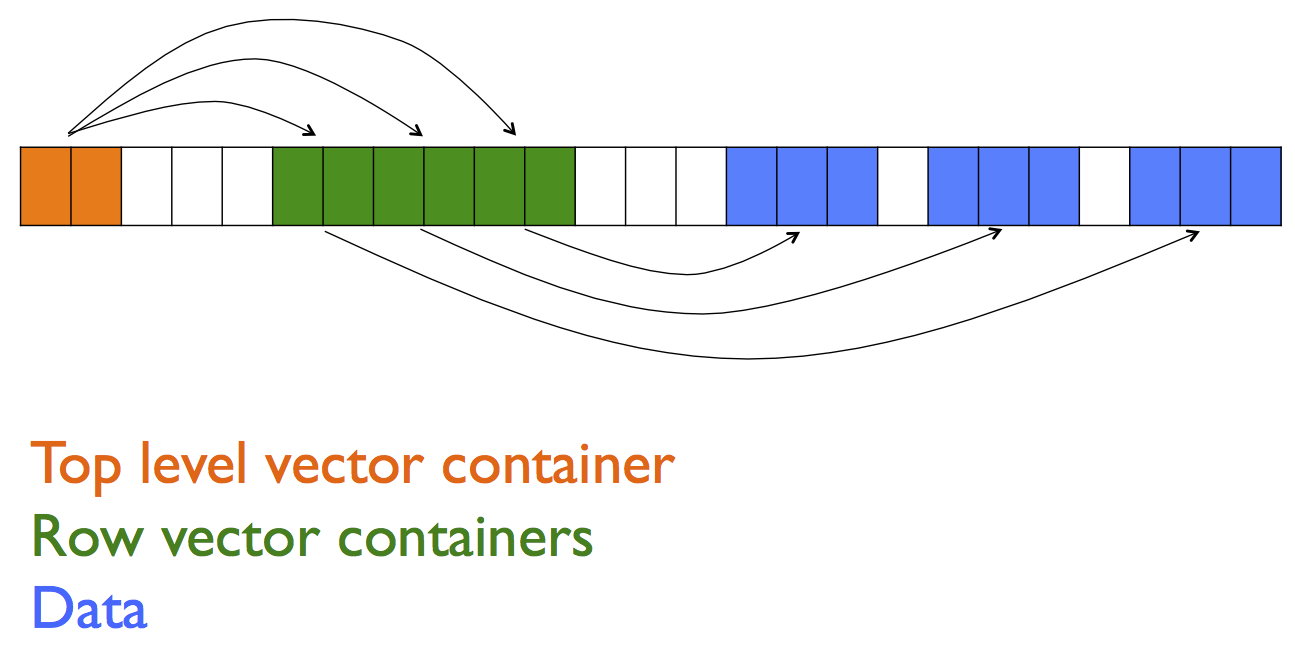
\includegraphics{fig/vector-of-vectors.png}
\caption{fig}
\end{figure}

\hypertarget{contiguous-memory}{%
\subsubsection{Contiguous memory}\label{contiguous-memory}}

\texttt{src/multi2.cpp}:

\begin{Shaded}
\begin{Highlighting}[]
\PreprocessorTok{#include }\ImportTok{<iostream>}
\PreprocessorTok{#include }\ImportTok{<vector>}

\DataTypeTok{int}\NormalTok{ main() \{}
  \DataTypeTok{unsigned} \DataTypeTok{int}\NormalTok{ nrows = }\DecValTok{3}\NormalTok{, ncols = }\DecValTok{3}\NormalTok{;}
  \BuiltInTok{std::}\NormalTok{vector<}\DataTypeTok{double}\NormalTok{> a;}
\NormalTok{  a.resize(nrows*ncols);}

  \DataTypeTok{double}\NormalTok{ n = }\FloatTok{0.}\NormalTok{;}
  \ControlFlowTok{for}\NormalTok{(}\DataTypeTok{unsigned} \DataTypeTok{int}\NormalTok{ i = }\DecValTok{0}\NormalTok{; i < nrows; i++) \{}
    \ControlFlowTok{for}\NormalTok{(}\DataTypeTok{unsigned} \DataTypeTok{int}\NormalTok{ j = }\DecValTok{0}\NormalTok{; j < ncols; j++) \{}
      \CommentTok{// manual indexing into "multi-dimensional array"}
\NormalTok{      a[i*ncols + j] = n;}
\NormalTok{      n++;}
\NormalTok{    \}}
\NormalTok{  \}}

  \ControlFlowTok{for}\NormalTok{(}\DataTypeTok{unsigned} \DataTypeTok{int}\NormalTok{ i = }\DecValTok{0}\NormalTok{; i < nrows*ncols; i++) \{}
    \BuiltInTok{std::}\NormalTok{cout << }\StringTok{"a["}\NormalTok{ << i << }\StringTok{"] = "}\NormalTok{ << a[i] << }\BuiltInTok{std::}\NormalTok{endl;}
\NormalTok{  \}}
  \ControlFlowTok{return} \DecValTok{0}\NormalTok{;}
\NormalTok{\}}
\end{Highlighting}
\end{Shaded}

Output:

\begin{verbatim}
$ clang++ -std=c++11 -Wall -Wextra -Wconversion src/multi2.cpp -o src/multi2
$ ./src/multi2
a[0] = 0
a[1] = 1
a[2] = 2
a[3] = 3
a[4] = 4
a[5] = 5
a[6] = 6
a[7] = 7
a[8] = 8
\end{verbatim}

\hypertarget{boost-multidimensional-array-library}{%
\subsection{Boost Multidimensional Array
Library}\label{boost-multidimensional-array-library}}

\texttt{src/array1.cpp}:

\begin{Shaded}
\begin{Highlighting}[]
\PreprocessorTok{#include }\ImportTok{<iostream>}
\PreprocessorTok{#include }\ImportTok{<boost/multi_array.hpp>}

\DataTypeTok{int}\NormalTok{ main() \{}
  \DataTypeTok{unsigned} \DataTypeTok{int}\NormalTok{ nrows = }\DecValTok{3}\NormalTok{, ncols = }\DecValTok{3}\NormalTok{;}
  \ExtensionTok{boost::}\NormalTok{multi_array<}\DataTypeTok{double}\NormalTok{, }\DecValTok{2}\NormalTok{> a(}\ExtensionTok{boost::}\NormalTok{extents[nrows][ncols]);}

  \DataTypeTok{double}\NormalTok{ n = }\FloatTok{0.}\NormalTok{;}
  \ControlFlowTok{for}\NormalTok{ (}\DataTypeTok{unsigned} \DataTypeTok{int}\NormalTok{ i = }\DecValTok{0}\NormalTok{; i < nrows; i++) \{}
    \ControlFlowTok{for}\NormalTok{ (}\DataTypeTok{unsigned} \DataTypeTok{int}\NormalTok{ j = }\DecValTok{0}\NormalTok{; j < ncols; j++) \{}
\NormalTok{      a[i][j] = n; }\CommentTok{// access elements like static array}
\NormalTok{      n++;}
\NormalTok{    \}}
\NormalTok{  \}}

  \ControlFlowTok{for}\NormalTok{ (}\DataTypeTok{unsigned} \DataTypeTok{int}\NormalTok{ i = }\DecValTok{0}\NormalTok{; i < nrows; i++) \{}
    \ControlFlowTok{for}\NormalTok{ (}\DataTypeTok{unsigned} \DataTypeTok{int}\NormalTok{ j = }\DecValTok{0}\NormalTok{; j < ncols; j++) \{}
      \BuiltInTok{std::}\NormalTok{cout << }\StringTok{"a["}\NormalTok{ << i << }\StringTok{"]["}\NormalTok{ << j << }\StringTok{"] = "}\NormalTok{ << a[i][j] << }\BuiltInTok{std::}\NormalTok{endl;}
\NormalTok{    \}}
\NormalTok{  \}}
  \ControlFlowTok{return} \DecValTok{0}\NormalTok{;}
\NormalTok{\}}
\end{Highlighting}
\end{Shaded}

Output:

\begin{verbatim}
$ clang++ -std=c++11 -Wall -Wextra -Wconversion src/array1.cpp -o src/array1
$ ./src/array1
a[0][0] = 0
a[0][1] = 1
a[0][2] = 2
a[1][0] = 3
a[1][1] = 4
a[1][2] = 5
a[2][0] = 6
a[2][1] = 7
a[2][2] = 8
\end{verbatim}

\hypertarget{accessing-the-contiguous-memory}{%
\subsubsection{Accessing the contiguous
memory}\label{accessing-the-contiguous-memory}}

\texttt{src/array2.cpp}:

\begin{Shaded}
\begin{Highlighting}[]
\PreprocessorTok{#include }\ImportTok{<iostream>}

\PreprocessorTok{#include }\ImportTok{<boost/multi_array.hpp>}

\DataTypeTok{int}\NormalTok{ main() \{}
  \ExtensionTok{boost::}\NormalTok{multi_array<}\DataTypeTok{double}\NormalTok{, }\DecValTok{2}\NormalTok{> a(}\ExtensionTok{boost::}\NormalTok{extents[}\DecValTok{3}\NormalTok{][}\DecValTok{3}\NormalTok{]);}

  \DataTypeTok{double}\NormalTok{ n = }\FloatTok{0.}\NormalTok{;}
  \ControlFlowTok{for}\NormalTok{ (}\DataTypeTok{unsigned} \DataTypeTok{int}\NormalTok{ i = }\DecValTok{0}\NormalTok{; i < }\DecValTok{3}\NormalTok{; i++) \{}
    \ControlFlowTok{for}\NormalTok{ (}\DataTypeTok{unsigned} \DataTypeTok{int}\NormalTok{ j = }\DecValTok{0}\NormalTok{; j < }\DecValTok{3}\NormalTok{; j++) \{}
\NormalTok{      a[i][j] = n;}
\NormalTok{      n++;}
\NormalTok{    \}}
\NormalTok{  \}}

  \ControlFlowTok{for}\NormalTok{ (}\DataTypeTok{unsigned} \DataTypeTok{int}\NormalTok{ n = }\DecValTok{0}\NormalTok{; n < a.num_elements(); n++) \{}
    \BuiltInTok{std::}\NormalTok{cout << }\StringTok{"a.data()["}\NormalTok{ << n << }\StringTok{"] = "}\NormalTok{ << a.data()[n] << }\BuiltInTok{std::}\NormalTok{endl;}
\NormalTok{  \}}

  \ControlFlowTok{return} \DecValTok{0}\NormalTok{;}
\NormalTok{\}}
\end{Highlighting}
\end{Shaded}

Output:

\begin{verbatim}
$ clang++ -std=c++11 -Wall -Wextra -Wconversion src/array2.cpp -o src/array2
$ ./src/array2
a.data()[0] = 0
a.data()[1] = 1
a.data()[2] = 2
a.data()[3] = 3
a.data()[4] = 4
a.data()[5] = 5
a.data()[6] = 6
a.data()[7] = 7
a.data()[8] = 8
\end{verbatim}

\hypertarget{performance}{%
\subsubsection{Performance}\label{performance}}

\texttt{src/perf1.cpp}:

\begin{Shaded}
\begin{Highlighting}[]
\PreprocessorTok{#include }\ImportTok{<iostream>}
\PreprocessorTok{#include }\ImportTok{<ctime>}
\PreprocessorTok{#include }\ImportTok{<boost/multi_array.hpp>}

\DataTypeTok{int}\NormalTok{ main() \{}
  \DataTypeTok{unsigned} \DataTypeTok{int}\NormalTok{ nrows = }\DecValTok{8192}\NormalTok{, ncols = }\DecValTok{8192}\NormalTok{;}
  \ExtensionTok{boost::}\NormalTok{multi_array<}\DataTypeTok{double}\NormalTok{, }\DecValTok{2}\NormalTok{> a(}\ExtensionTok{boost::}\NormalTok{extents[nrows][ncols]);}

  \ControlFlowTok{for}\NormalTok{ (}\DataTypeTok{unsigned} \DataTypeTok{int}\NormalTok{ i = }\DecValTok{0}\NormalTok{; i < nrows; i++) \{}
    \ControlFlowTok{for}\NormalTok{ (}\DataTypeTok{unsigned} \DataTypeTok{int}\NormalTok{ j = }\DecValTok{0}\NormalTok{; j < ncols; j++) \{}
\NormalTok{      a[i][j] = }\FloatTok{1.0}\NormalTok{;}
\NormalTok{    \}}
\NormalTok{  \}}
  
  \KeywordTok{auto}\NormalTok{ t0 = }\BuiltInTok{std::}\NormalTok{clock();}
  \DataTypeTok{double}\NormalTok{ sum = }\FloatTok{0.}\NormalTok{;}
  \ControlFlowTok{for}\NormalTok{ (}\DataTypeTok{unsigned} \DataTypeTok{int}\NormalTok{ i = }\DecValTok{0}\NormalTok{; i < nrows; i++) \{}
    \ControlFlowTok{for}\NormalTok{ (}\DataTypeTok{unsigned} \DataTypeTok{int}\NormalTok{ j = }\DecValTok{0}\NormalTok{; j < ncols; j++) \{}
\NormalTok{      sum += a[i][j];}
\NormalTok{    \}}
\NormalTok{  \}}
  \KeywordTok{auto}\NormalTok{ t1 = }\BuiltInTok{std::}\NormalTok{clock();}

  \BuiltInTok{std::}\NormalTok{cout << }\StringTok{" boost: sum = "}\NormalTok{ << sum << }\StringTok{", time = "}
\NormalTok{            << }\DataTypeTok{double}\NormalTok{(t1-t0) / CLOCKS_PER_SEC}
\NormalTok{            << }\StringTok{" seconds"}\NormalTok{<< }\BuiltInTok{std::}\NormalTok{endl;}

  \KeywordTok{auto}\NormalTok{ b = a.data();}
\NormalTok{  t0 = }\BuiltInTok{std::}\NormalTok{clock();}
\NormalTok{  sum = }\FloatTok{0.}\NormalTok{;}
  \ControlFlowTok{for}\NormalTok{ (}\DataTypeTok{unsigned} \DataTypeTok{int}\NormalTok{ n = }\DecValTok{0}\NormalTok{; n < nrows*ncols; n++) \{}
\NormalTok{    sum += b[n];}
\NormalTok{  \}}
\NormalTok{  t1 = }\BuiltInTok{std::}\NormalTok{clock();}
  \BuiltInTok{std::}\NormalTok{cout << }\StringTok{"direct: sum = "}\NormalTok{ << sum << }\StringTok{", time = "}
\NormalTok{            << }\DataTypeTok{double}\NormalTok{(t1-t0) / CLOCKS_PER_SEC}
\NormalTok{            << }\StringTok{" seconds"}\NormalTok{<< }\BuiltInTok{std::}\NormalTok{endl;}
  \ControlFlowTok{return} \DecValTok{0}\NormalTok{;}
\NormalTok{\}}
\end{Highlighting}
\end{Shaded}

Output:

\begin{verbatim}
$ clang++ -std=c++11 -Wall -Wextra -Wconversion src/perf1.cpp -o src/perf1
$ ./src/perf1
 boost: sum = 6.71089e+07, time = 4.55984 seconds
direct: sum = 6.71089e+07, time = 0.240126 seconds
$ ./src/perf1
 boost: sum = 6.71089e+07, time = 4.41117 seconds
direct: sum = 6.71089e+07, time = 0.228782 seconds
$ ./src/perf1
 boost: sum = 6.71089e+07, time = 4.38506 seconds
direct: sum = 6.71089e+07, time = 0.235112 seconds
\end{verbatim}

\hypertarget{performance-1}{%
\subsubsection{Performance}\label{performance-1}}

From \texttt{src/perf2.cpp}:

\begin{Shaded}
\begin{Highlighting}[]
\CommentTok{// disable boost range checking}
\PreprocessorTok{#define B}\NormalTok{OOST_DISABLE_ASSERTS}
\PreprocessorTok{#include }\ImportTok{<boost/multi_array.hpp>}
\end{Highlighting}
\end{Shaded}

Output:

\begin{verbatim}
$ clang++ -std=c++11 -Wall -Wextra -Wconversion src/perf2.cpp -o src/perf2
$ ./src/perf2
 boost: sum = 6.71089e+07, time = 4.4622 seconds
direct: sum = 6.71089e+07, time = 0.235016 seconds
$ ./src/perf2
 boost: sum = 6.71089e+07, time = 4.26261 seconds
direct: sum = 6.71089e+07, time = 0.226978 seconds
$ ./src/perf2
 boost: sum = 6.71089e+07, time = 4.2159 seconds
direct: sum = 6.71089e+07, time = 0.240271 seconds
\end{verbatim}

\hypertarget{compiler-optimization}{%
\subsubsection{Compiler optimization}\label{compiler-optimization}}

Enable compiler optimizations with the \texttt{-O3} argument.

With range checking:

Output:

\begin{verbatim}
$ clang++ -O3 -std=c++11 -Wall -Wextra -Wconversion src/perf1.cpp -o src/perf1
$ ./src/perf1
 boost: sum = 6.71089e+07, time = 0.102904 seconds
direct: sum = 6.71089e+07, time = 0.107179 seconds
$ ./src/perf1
 boost: sum = 6.71089e+07, time = 0.119958 seconds
direct: sum = 6.71089e+07, time = 0.121643 seconds
$ ./src/perf1
 boost: sum = 6.71089e+07, time = 0.10259 seconds
direct: sum = 6.71089e+07, time = 0.105372 seconds
\end{verbatim}

Range checking disabled:

Output:

\begin{verbatim}
$ clang++ -O3 -std=c++11 -Wall -Wextra -Wconversion src/perf2.cpp -o src/perf2
$ ./src/perf2
 boost: sum = 6.71089e+07, time = 0.102209 seconds
direct: sum = 6.71089e+07, time = 0.102016 seconds
$ ./src/perf2
 boost: sum = 6.71089e+07, time = 0.104234 seconds
direct: sum = 6.71089e+07, time = 0.105256 seconds
$ ./src/perf2
 boost: sum = 6.71089e+07, time = 0.101876 seconds
direct: sum = 6.71089e+07, time = 0.117592 seconds
\end{verbatim}

\hypertarget{range-checking}{%
\subsubsection{Range checking}\label{range-checking}}

\texttt{src/array3a.cpp}:

\begin{Shaded}
\begin{Highlighting}[]
\PreprocessorTok{#include }\ImportTok{<iostream>}
\PreprocessorTok{#include }\ImportTok{<boost/multi_array.hpp>}

\DataTypeTok{int}\NormalTok{ main() \{}
  \ExtensionTok{boost::}\NormalTok{multi_array<}\DataTypeTok{double}\NormalTok{, }\DecValTok{2}\NormalTok{> a(}\ExtensionTok{boost::}\NormalTok{extents[}\DecValTok{3}\NormalTok{][}\DecValTok{3}\NormalTok{]);}
\NormalTok{  a[}\DecValTok{3}\NormalTok{][}\DecValTok{3}\NormalTok{] = }\FloatTok{1.}\NormalTok{;}
  \ControlFlowTok{return} \DecValTok{0}\NormalTok{;}
\NormalTok{\}}
\end{Highlighting}
\end{Shaded}

Output:

\begin{verbatim}
$ clang++ -std=c++11 -Wall -Wextra -Wconversion src/array3a.cpp -o src/array3a
$ ./src/array3a
Assertion failed: (size_type(idx - index_bases[0]) < extents[0]), function access, file /usr/local/include/boost/multi_array/base.hpp, line 136.
\end{verbatim}

\hypertarget{range-checking-1}{%
\subsubsection{Range checking}\label{range-checking-1}}

\texttt{src/array3b.cpp}:

\begin{Shaded}
\begin{Highlighting}[]
\PreprocessorTok{#include }\ImportTok{<iostream>}
\PreprocessorTok{#define B}\NormalTok{OOST_DISABLE_ASSERTS}
\PreprocessorTok{#include }\ImportTok{<boost/multi_array.hpp>}

\DataTypeTok{int}\NormalTok{ main() \{}
  \ExtensionTok{boost::}\NormalTok{multi_array<}\DataTypeTok{double}\NormalTok{, }\DecValTok{2}\NormalTok{> a(}\ExtensionTok{boost::}\NormalTok{extents[}\DecValTok{3}\NormalTok{][}\DecValTok{3}\NormalTok{]);}
\NormalTok{  a[}\DecValTok{3}\NormalTok{][}\DecValTok{3}\NormalTok{] = }\FloatTok{1.}\NormalTok{;}
  \ControlFlowTok{return} \DecValTok{0}\NormalTok{;}
\NormalTok{\}}
\end{Highlighting}
\end{Shaded}

Output:

\begin{verbatim}
$ clang++ -std=c++11 -Wall -Wextra -Wconversion src/array3b.cpp -o src/array3b
$ ./src/array3b
$ clang++ -std=c++11 -g -fsanitize=address -Wall -Wextra -Wconversion src/array3b.cpp -o src/array3b
$ ./src/array3b
=================================================================
==36808==ERROR: AddressSanitizer: heap-buffer-overflow on address 0x60700000df30 at pc 0x00010dc1aad5 bp 0x7fff51fe67d0 sp 0x7fff51fe67c8
WRITE of size 8 at 0x60700000df30 thread T0
    #0 0x10dc1aad4 in main array3b.cpp:7
    #1 0x7fff9426d5ac in start (libdyld.dylib+0x35ac)
    #2 0x0  (<unknown module>)

0x60700000df30 is located 16 bytes to the left of 67-byte region [0x60700000df40,0x60700000df83)
allocated by thread T0 here:
    #0 0x10dc759c0 in wrap_malloc (libclang_rt.asan_osx_dynamic.dylib+0x489c0)
    #1 0x7fff9283364d in _xpc_malloc (libxpc.dylib+0x264d)
    #2 0x7fff92833529 in _xpc_dictionary_insert (libxpc.dylib+0x2529)
    #3 0x7fff92833325 in xpc_dictionary_set_string (libxpc.dylib+0x2325)
    #4 0x7fff9283319c in _xpc_collect_environment (libxpc.dylib+0x219c)
    #5 0x7fff92832d41 in _libxpc_initializer (libxpc.dylib+0x1d41)
    #6 0x7fff924bfa06 in libSystem_initializer (libSystem.B.dylib+0x1a06)
    #7 0x7fff6536e10a  (<unknown module>)
    #8 0x7fff6536e283  (<unknown module>)
    #9 0x7fff6536a8bc  (<unknown module>)
    #10 0x7fff6536a851  (<unknown module>)
    #11 0x7fff6536a851  (<unknown module>)
    #12 0x7fff6536a851  (<unknown module>)
    #13 0x7fff6536a742  (<unknown module>)
    #14 0x7fff6536a9b2  (<unknown module>)
    #15 0x7fff6535d0f0  (<unknown module>)
    #16 0x7fff65360d97  (<unknown module>)
    #17 0x7fff6535c275  (<unknown module>)
    #18 0x7fff6535c035  (<unknown module>)
    #19 0x0  (<unknown module>)

SUMMARY: AddressSanitizer: heap-buffer-overflow array3b.cpp:7 in main
Shadow bytes around the buggy address:
  0x1c0e00001b90: fa fa fa fa fa fa fa fa fa fa fa fa fa fa fa fa
  0x1c0e00001ba0: fa fa fa fa fa fa fa fa fa fa fa fa fa fa fa fa
  0x1c0e00001bb0: fa fa fa fa fa fa fa fa fa fa fa fa fa fa fa fa
  0x1c0e00001bc0: fa fa fa fa fa fa fa fa fa fa fa fa fa fa fa fa
  0x1c0e00001bd0: fa fa fa fa fa fa fa fa fa fa 00 00 00 00 00 00
=>0x1c0e00001be0: 00 00 00 fa fa fa[fa]fa 00 00 00 00 00 00 00 00
  0x1c0e00001bf0: 03 fa fa fa fa fa 00 00 00 00 00 00 00 00 00 fa
  0x1c0e00001c00: fa fa fa fa fa fa fa fa fa fa fa fa fa fa fa fa
  0x1c0e00001c10: fa fa fa fa fa fa fa fa fa fa fa fa fa fa fa fa
  0x1c0e00001c20: fa fa fa fa fa fa fa fa fa fa fa fa fa fa fa fa
  0x1c0e00001c30: fa fa fa fa fa fa fa fa fa fa fa fa fa fa fa fa
Shadow byte legend (one shadow byte represents 8 application bytes):
  Addressable:           00
  Partially addressable: 01 02 03 04 05 06 07 
  Heap left redzone:       fa
  Heap right redzone:      fb
  Freed heap region:       fd
  Stack left redzone:      f1
  Stack mid redzone:       f2
  Stack right redzone:     f3
  Stack partial redzone:   f4
  Stack after return:      f5
  Stack use after scope:   f8
  Global redzone:          f9
  Global init order:       f6
  Poisoned by user:        f7
  Container overflow:      fc
  Array cookie:            ac
  Intra object redzone:    bb
  ASan internal:           fe
  Left alloca redzone:     ca
  Right alloca redzone:    cb
==36808==ABORTING
\end{verbatim}

\hypertarget{range-checking-2}{%
\subsubsection{Range checking}\label{range-checking-2}}

Another method to check for memory leaks is \texttt{valgrind}.

Output:

\begin{verbatim}
$ clang++ -g -Wall -Wextra -Wconversion src/array3b.cpp -o src/array3b
$ valgrind ./src/array3b
==36817== Memcheck, a memory error detector
==36817== Copyright (C) 2002-2015, and GNU GPL'd, by Julian Seward et al.
==36817== Using Valgrind-3.12.0 and LibVEX; rerun with -h for copyright info
==36817== Command: ./src/array3b
==36817== 
==36817== Invalid write of size 8
==36817==    at 0x10000109D: main (array3b.cpp:7)
==36817==  Address 0x100a88180 is 16 bytes after a block of size 80 in arena "client"
==36817== 
==36817== 
==36817== HEAP SUMMARY:
==36817==     in use at exit: 22,458 bytes in 194 blocks
==36817==   total heap usage: 258 allocs, 64 frees, 28,226 bytes allocated
==36817== 
==36817== LEAK SUMMARY:
==36817==    definitely lost: 0 bytes in 0 blocks
==36817==    indirectly lost: 0 bytes in 0 blocks
==36817==      possibly lost: 2,064 bytes in 1 blocks
==36817==    still reachable: 0 bytes in 0 blocks
==36817==         suppressed: 20,394 bytes in 193 blocks
==36817== Rerun with --leak-check=full to see details of leaked memory
==36817== 
==36817== For counts of detected and suppressed errors, rerun with: -v
==36817== ERROR SUMMARY: 1 errors from 1 contexts (suppressed: 0 from 0)
\end{verbatim}

\hypertarget{elementwise-comparison}{%
\subsubsection{Elementwise comparison}\label{elementwise-comparison}}

\texttt{src/array5.cpp}:

\begin{Shaded}
\begin{Highlighting}[]
\PreprocessorTok{#include }\ImportTok{<iostream>}
\PreprocessorTok{#include }\ImportTok{<boost/multi_array.hpp>}

\DataTypeTok{int}\NormalTok{ main() \{}
  \ExtensionTok{boost::}\NormalTok{multi_array<}\DataTypeTok{double}\NormalTok{, }\DecValTok{2}\NormalTok{> a(}\ExtensionTok{boost::}\NormalTok{extents[}\DecValTok{3}\NormalTok{][}\DecValTok{3}\NormalTok{]);}
  \ExtensionTok{boost::}\NormalTok{multi_array<}\DataTypeTok{double}\NormalTok{, }\DecValTok{2}\NormalTok{> b(}\ExtensionTok{boost::}\NormalTok{extents[}\DecValTok{3}\NormalTok{][}\DecValTok{3}\NormalTok{]);}

  \ControlFlowTok{for}\NormalTok{ (}\DataTypeTok{unsigned} \DataTypeTok{int}\NormalTok{ i = }\DecValTok{0}\NormalTok{; i < }\DecValTok{3}\NormalTok{; i++) \{}
    \ControlFlowTok{for}\NormalTok{ (}\DataTypeTok{unsigned} \DataTypeTok{int}\NormalTok{ j = }\DecValTok{0}\NormalTok{; j < }\DecValTok{3}\NormalTok{; j++) \{}
\NormalTok{      a[i][j] = }\FloatTok{1.}\NormalTok{;}
\NormalTok{      b[i][j] = }\FloatTok{2.}\NormalTok{;}
\NormalTok{    \}}
\NormalTok{  \}}

  \BuiltInTok{std::}\NormalTok{cout << }\StringTok{"a == b: "}\NormalTok{ << (a == b) << }\BuiltInTok{std::}\NormalTok{endl;}
  \BuiltInTok{std::}\NormalTok{cout << }\StringTok{"a < b: "}\NormalTok{ << (a < b) << }\BuiltInTok{std::}\NormalTok{endl;}
  \BuiltInTok{std::}\NormalTok{cout << }\StringTok{"a > b: "}\NormalTok{ << (a > b) << }\BuiltInTok{std::}\NormalTok{endl;}

  \ControlFlowTok{return} \DecValTok{0}\NormalTok{;}
\NormalTok{\}}
\end{Highlighting}
\end{Shaded}

Output:

\begin{verbatim}
$ clang++ -std=c++11 -Wall -Wextra -Wconversion src/array5.cpp -o src/array5
$ ./src/array5
a == b: 0
a < b: 1
a > b: 0
\end{verbatim}

\hypertarget{copy-or-reference}{%
\subsubsection{Copy or reference?}\label{copy-or-reference}}

\texttt{src/array6a.cpp}:

\begin{Shaded}
\begin{Highlighting}[]
\PreprocessorTok{#include }\ImportTok{<iostream>}
\PreprocessorTok{#include }\ImportTok{<boost/multi_array.hpp>}

\DataTypeTok{int}\NormalTok{ main() \{}
  \ExtensionTok{boost::}\NormalTok{multi_array<}\DataTypeTok{double}\NormalTok{, }\DecValTok{2}\NormalTok{> a(}\ExtensionTok{boost::}\NormalTok{extents[}\DecValTok{3}\NormalTok{][}\DecValTok{3}\NormalTok{]);}

  \ControlFlowTok{for}\NormalTok{ (}\DataTypeTok{unsigned} \DataTypeTok{int}\NormalTok{ i = }\DecValTok{0}\NormalTok{; i < }\DecValTok{3}\NormalTok{; i++) \{}
    \ControlFlowTok{for}\NormalTok{ (}\DataTypeTok{unsigned} \DataTypeTok{int}\NormalTok{ j = }\DecValTok{0}\NormalTok{; j < }\DecValTok{3}\NormalTok{; j++) \{}
\NormalTok{      a[i][j] = }\FloatTok{1.}\NormalTok{;}
\NormalTok{    \}}
\NormalTok{  \}}

  \KeywordTok{auto}\NormalTok{ b = a; }\CommentTok{// copy or reference?}

  \ControlFlowTok{for}\NormalTok{ (}\DataTypeTok{unsigned} \DataTypeTok{int}\NormalTok{ i = }\DecValTok{0}\NormalTok{; i < }\DecValTok{3}\NormalTok{; i++) \{}
    \ControlFlowTok{for}\NormalTok{ (}\DataTypeTok{unsigned} \DataTypeTok{int}\NormalTok{ j = }\DecValTok{0}\NormalTok{; j < }\DecValTok{3}\NormalTok{; j++) \{}
\NormalTok{      a[i][j] = }\FloatTok{2.}\NormalTok{;}
\NormalTok{    \}}
\NormalTok{  \}}

  \BuiltInTok{std::}\NormalTok{cout << }\StringTok{"a b"}\NormalTok{ << }\BuiltInTok{std::}\NormalTok{endl;}
  \BuiltInTok{std::}\NormalTok{cout << }\StringTok{"---"}\NormalTok{ << }\BuiltInTok{std::}\NormalTok{endl;}
  \ControlFlowTok{for}\NormalTok{ (}\DataTypeTok{unsigned} \DataTypeTok{int}\NormalTok{ i = }\DecValTok{0}\NormalTok{; i < }\DecValTok{3}\NormalTok{; i++) \{}
    \ControlFlowTok{for}\NormalTok{ (}\DataTypeTok{unsigned} \DataTypeTok{int}\NormalTok{ j = }\DecValTok{0}\NormalTok{; j < }\DecValTok{3}\NormalTok{; j++) \{}
      \BuiltInTok{std::}\NormalTok{cout << a[i][j] << }\StringTok{" "}\NormalTok{ << b[i][j] << }\BuiltInTok{std::}\NormalTok{endl;}
\NormalTok{    \}}
\NormalTok{  \}}
  \ControlFlowTok{return} \DecValTok{0}\NormalTok{;}
\NormalTok{\}}
\end{Highlighting}
\end{Shaded}

Output:

\begin{verbatim}
$ clang++ -std=c++11 -Wall -Wextra -Wconversion src/array6a.cpp -o src/array6a
$ ./src/array6a
a b
---
2 1
2 1
2 1
2 1
2 1
2 1
2 1
2 1
2 1
\end{verbatim}

\hypertarget{passing-an-array-to-a-function}{%
\subsubsection{Passing an array to a
function}\label{passing-an-array-to-a-function}}

\texttt{src/array6b.cpp}:

\begin{Shaded}
\begin{Highlighting}[]
\PreprocessorTok{#include }\ImportTok{<iostream>}
\PreprocessorTok{#include }\ImportTok{<boost/multi_array.hpp>}

\DataTypeTok{void}\NormalTok{ increment(}\ExtensionTok{boost::}\NormalTok{multi_array<}\DataTypeTok{double}\NormalTok{, }\DecValTok{2}\NormalTok{> b) \{}
  \ControlFlowTok{for}\NormalTok{ (}\DataTypeTok{unsigned} \DataTypeTok{int}\NormalTok{ i = }\DecValTok{0}\NormalTok{; i < }\DecValTok{3}\NormalTok{; i++) \{}
    \ControlFlowTok{for}\NormalTok{ (}\DataTypeTok{unsigned} \DataTypeTok{int}\NormalTok{ j = }\DecValTok{0}\NormalTok{; j < }\DecValTok{3}\NormalTok{; j++) \{}
\NormalTok{      b[i][j]++;}
\NormalTok{    \}}
\NormalTok{  \}}
\NormalTok{\}}

\DataTypeTok{int}\NormalTok{ main() \{}
  \ExtensionTok{boost::}\NormalTok{multi_array<}\DataTypeTok{double}\NormalTok{, }\DecValTok{2}\NormalTok{> a(}\ExtensionTok{boost::}\NormalTok{extents[}\DecValTok{3}\NormalTok{][}\DecValTok{3}\NormalTok{]);}

  \ControlFlowTok{for}\NormalTok{ (}\DataTypeTok{unsigned} \DataTypeTok{int}\NormalTok{ i = }\DecValTok{0}\NormalTok{; i < }\DecValTok{3}\NormalTok{; i++) \{}
    \ControlFlowTok{for}\NormalTok{ (}\DataTypeTok{unsigned} \DataTypeTok{int}\NormalTok{ j = }\DecValTok{0}\NormalTok{; j < }\DecValTok{3}\NormalTok{; j++) \{}
\NormalTok{      a[i][j] = }\FloatTok{1.}\NormalTok{;}
\NormalTok{    \}}
\NormalTok{  \}}

\NormalTok{  increment(a);}

  \ControlFlowTok{for}\NormalTok{ (}\DataTypeTok{unsigned} \DataTypeTok{int}\NormalTok{ i = }\DecValTok{0}\NormalTok{; i < }\DecValTok{3}\NormalTok{; i++) \{}
    \ControlFlowTok{for}\NormalTok{ (}\DataTypeTok{unsigned} \DataTypeTok{int}\NormalTok{ j = }\DecValTok{0}\NormalTok{; j < }\DecValTok{3}\NormalTok{; j++) \{}
      \BuiltInTok{std::}\NormalTok{cout << a[i][j] << }\BuiltInTok{std::}\NormalTok{endl;}
\NormalTok{    \}}
\NormalTok{  \}}
  \ControlFlowTok{return} \DecValTok{0}\NormalTok{;}
\NormalTok{\}}
\end{Highlighting}
\end{Shaded}

Output:

\begin{verbatim}
$ clang++ -std=c++11 -Wall -Wextra -Wconversion src/array6b.cpp -o src/array6b
$ ./src/array6b
1
1
1
1
1
1
1
1
1
\end{verbatim}

\hypertarget{passing-by-reference}{%
\subsubsection{Passing by reference}\label{passing-by-reference}}

From \texttt{src/array6c.cpp}:

\begin{Shaded}
\begin{Highlighting}[]
\DataTypeTok{void}\NormalTok{ increment(}\ExtensionTok{boost::}\NormalTok{multi_array<}\DataTypeTok{double}\NormalTok{, }\DecValTok{2}\NormalTok{>& b) \{}
  \ControlFlowTok{for}\NormalTok{ (}\DataTypeTok{unsigned} \DataTypeTok{int}\NormalTok{ i = }\DecValTok{0}\NormalTok{; i < }\DecValTok{3}\NormalTok{; i++) \{}
    \ControlFlowTok{for}\NormalTok{ (}\DataTypeTok{unsigned} \DataTypeTok{int}\NormalTok{ j = }\DecValTok{0}\NormalTok{; j < }\DecValTok{3}\NormalTok{; j++) \{}
\NormalTok{      b[i][j]++;}
\NormalTok{    \}}
\NormalTok{  \}}
\NormalTok{\}}
\end{Highlighting}
\end{Shaded}

Output:

\begin{verbatim}
$ clang++ -std=c++11 -Wall -Wextra -Wconversion src/array6c.cpp -o src/array6c
$ ./src/array6c
2
2
2
2
2
2
2
2
2
\end{verbatim}

\hypertarget{array-operations}{%
\subsubsection{Array operations?}\label{array-operations}}

\begin{itemize}
\item
  Boost \texttt{multi\_array} does not support array operations like
  NumPy
\item
  If \texttt{a} is a \texttt{multi\_array} things like \texttt{2*a} and
  \texttt{a\ =\ 1.0} will not work and will lead to very long compiler
  error messages.
\item
  If you want this kind of stuff, have a look at:

  \begin{itemize}
  \item
    http://eigen.tuxfamily.org/index.php?title=Main\_Page
  \item
    http://arma.sourceforge.net/
  \item
    https://github.com/arrayfire/arrayfire
  \end{itemize}
\end{itemize}

\hypertarget{array-views}{%
\subsubsection{Array views}\label{array-views}}

An \textbf{array view} is essentially a reference into a sub-array of a
larger array.

\texttt{src/array9.cpp}:

\begin{Shaded}
\begin{Highlighting}[]
\PreprocessorTok{#include }\ImportTok{<iostream>}
\PreprocessorTok{#include }\ImportTok{<boost/multi_array.hpp>}

\DataTypeTok{int}\NormalTok{ main() \{}
  \ExtensionTok{boost::}\NormalTok{multi_array<}\DataTypeTok{double}\NormalTok{, }\DecValTok{2}\NormalTok{> a(}\ExtensionTok{boost::}\NormalTok{extents[}\DecValTok{3}\NormalTok{][}\DecValTok{3}\NormalTok{]);}

  \DataTypeTok{double}\NormalTok{ n = }\FloatTok{0.}\NormalTok{;}
  \ControlFlowTok{for}\NormalTok{ (}\DataTypeTok{unsigned} \DataTypeTok{int}\NormalTok{ i = }\DecValTok{0}\NormalTok{; i < }\DecValTok{3}\NormalTok{; i++) \{}
    \ControlFlowTok{for}\NormalTok{ (}\DataTypeTok{unsigned} \DataTypeTok{int}\NormalTok{ j = }\DecValTok{0}\NormalTok{; j < }\DecValTok{3}\NormalTok{; j++) \{}
\NormalTok{      a[i][j] = n;}
\NormalTok{      n++;}
\NormalTok{    \}}
\NormalTok{  \}}

  \CommentTok{/* Setup b as a view into a subset of a. */}
  \KeywordTok{typedef} \ExtensionTok{boost::}\NormalTok{multi_array<}\DataTypeTok{double}\NormalTok{, }\DecValTok{2}\NormalTok{>::index_range index_range;}
  \KeywordTok{auto}\NormalTok{ b = a[}\ExtensionTok{boost::}\NormalTok{indices[index_range(}\DecValTok{1}\NormalTok{,}\DecValTok{3}\NormalTok{)][index_range(}\DecValTok{1}\NormalTok{,}\DecValTok{3}\NormalTok{)]];}

  \ControlFlowTok{for}\NormalTok{ (}\DataTypeTok{unsigned} \DataTypeTok{int}\NormalTok{ i = }\DecValTok{0}\NormalTok{; i < }\DecValTok{2}\NormalTok{; i++) \{}
    \ControlFlowTok{for}\NormalTok{ (}\DataTypeTok{unsigned} \DataTypeTok{int}\NormalTok{ j = }\DecValTok{0}\NormalTok{; j < }\DecValTok{2}\NormalTok{; j++) \{}
\NormalTok{      b[i][j] = -}\FloatTok{1.}\NormalTok{;}
\NormalTok{    \}}
\NormalTok{  \}}

  \ControlFlowTok{for}\NormalTok{ (}\DataTypeTok{unsigned} \DataTypeTok{int}\NormalTok{ i = }\DecValTok{0}\NormalTok{; i < }\DecValTok{3}\NormalTok{; i++) \{}
    \ControlFlowTok{for}\NormalTok{ (}\DataTypeTok{unsigned} \DataTypeTok{int}\NormalTok{ j = }\DecValTok{0}\NormalTok{; j < }\DecValTok{3}\NormalTok{; j++) \{}
      \BuiltInTok{std::}\NormalTok{cout << a[i][j] << }\BuiltInTok{std::}\NormalTok{endl;}
\NormalTok{    \}}
\NormalTok{  \}}
  \ControlFlowTok{return} \DecValTok{0}\NormalTok{;}
\NormalTok{\}}
\end{Highlighting}
\end{Shaded}

Output:

\begin{verbatim}
$ clang++ -std=c++11 -Wall -Wextra -Wconversion src/array9.cpp -o src/array9
$ ./src/array9
0
1
2
3
-1
-1
6
-1
-1
\end{verbatim}

\hypertarget{storage-order}{%
\subsubsection{Storage order}\label{storage-order}}

\texttt{src/array10a.cpp}:

\begin{Shaded}
\begin{Highlighting}[]
\PreprocessorTok{#include }\ImportTok{<iostream>}
\PreprocessorTok{#include }\ImportTok{<boost/multi_array.hpp>}

\DataTypeTok{int}\NormalTok{ main() \{}
  \ExtensionTok{boost::}\NormalTok{multi_array<}\DataTypeTok{double}\NormalTok{, }\DecValTok{2}\NormalTok{> a(}\ExtensionTok{boost::}\NormalTok{extents[}\DecValTok{3}\NormalTok{][}\DecValTok{3}\NormalTok{]);}

  \DataTypeTok{double}\NormalTok{ n = }\FloatTok{0.}\NormalTok{;}
  \ControlFlowTok{for}\NormalTok{ (}\DataTypeTok{unsigned} \DataTypeTok{int}\NormalTok{ i = }\DecValTok{0}\NormalTok{; i < }\DecValTok{3}\NormalTok{; i++) \{}
    \ControlFlowTok{for}\NormalTok{ (}\DataTypeTok{unsigned} \DataTypeTok{int}\NormalTok{ j = }\DecValTok{0}\NormalTok{; j < }\DecValTok{3}\NormalTok{; j++) \{}
\NormalTok{      a[i][j] = n;}
\NormalTok{      n++;}
\NormalTok{    \}}
\NormalTok{  \}}

  \KeywordTok{auto}\NormalTok{ b = a.data();}
  \ControlFlowTok{for}\NormalTok{ (}\DataTypeTok{unsigned} \DataTypeTok{int}\NormalTok{ n = }\DecValTok{0}\NormalTok{; n < a.num_elements(); n++) \{}
    \BuiltInTok{std::}\NormalTok{cout << }\StringTok{"b["}\NormalTok{ << n << }\StringTok{"] = "}\NormalTok{ << b[n] << }\BuiltInTok{std::}\NormalTok{endl;}
\NormalTok{  \}}

  \ControlFlowTok{return} \DecValTok{0}\NormalTok{;}
\NormalTok{\}}
\end{Highlighting}
\end{Shaded}

Output:

\begin{verbatim}
$ clang++ -std=c++11 -Wall -Wextra -Wconversion src/array10a.cpp -o src/array10a
$ ./src/array10a
b[0] = 0
b[1] = 1
b[2] = 2
b[3] = 3
b[4] = 4
b[5] = 5
b[6] = 6
b[7] = 7
b[8] = 8
\end{verbatim}

\begin{itemize}
\item
  Uses C convention that rows are stored contiguously in memory (row
  major order)
\item
  Or put another way, the last index in a multidimensional array changes
  fastest when traversing through linear memory
\end{itemize}

\hypertarget{fortran-storage-order}{%
\subsubsection{``Fortran'' storage order}\label{fortran-storage-order}}

\texttt{src/array10b.cpp}:

\begin{Shaded}
\begin{Highlighting}[]
\PreprocessorTok{#include }\ImportTok{<iostream>}
\PreprocessorTok{#include }\ImportTok{<boost/multi_array.hpp>}

\DataTypeTok{int}\NormalTok{ main() \{}
  \ExtensionTok{boost::}\NormalTok{multi_array<}\DataTypeTok{double}\NormalTok{, }\DecValTok{2}\NormalTok{> a(}\ExtensionTok{boost::}\NormalTok{extents[}\DecValTok{3}\NormalTok{][}\DecValTok{3}\NormalTok{],}
                                  \ExtensionTok{boost::}\NormalTok{fortran_storage_order());}

  \DataTypeTok{double}\NormalTok{ n = }\FloatTok{0.}\NormalTok{;}
  \ControlFlowTok{for}\NormalTok{ (}\DataTypeTok{unsigned} \DataTypeTok{int}\NormalTok{ i = }\DecValTok{0}\NormalTok{; i < }\DecValTok{3}\NormalTok{; i++) \{}
    \ControlFlowTok{for}\NormalTok{ (}\DataTypeTok{unsigned} \DataTypeTok{int}\NormalTok{ j = }\DecValTok{0}\NormalTok{; j < }\DecValTok{3}\NormalTok{; j++) \{}
\NormalTok{      a[i][j] = n;}
\NormalTok{      n++;}
\NormalTok{    \}}
\NormalTok{  \}}

  \KeywordTok{auto}\NormalTok{ b = a.data();}
  \ControlFlowTok{for}\NormalTok{ (}\DataTypeTok{unsigned} \DataTypeTok{int}\NormalTok{ n = }\DecValTok{0}\NormalTok{; n < a.num_elements(); n++) \{}
    \BuiltInTok{std::}\NormalTok{cout << }\StringTok{"b["}\NormalTok{ << n << }\StringTok{"] = "}\NormalTok{ << b[n] << }\BuiltInTok{std::}\NormalTok{endl;}
\NormalTok{  \}}

  \ControlFlowTok{return} \DecValTok{0}\NormalTok{;}
\NormalTok{\}}
\end{Highlighting}
\end{Shaded}

Output:

\begin{verbatim}
$ clang++ -std=c++11 -Wall -Wextra -Wconversion src/array10b.cpp -o src/array10b
$ ./src/array10b
b[0] = 0
b[1] = 3
b[2] = 6
b[3] = 1
b[4] = 4
b[5] = 7
b[6] = 2
b[7] = 5
b[8] = 8
\end{verbatim}

\begin{itemize}
\item
  In Fortran columns are stored contiguously in memory (column major
  order)
\item
  Or put another way, the first index in a multidimensional array
  changes fastest when traversing through linear memory
\end{itemize}

\hypertarget{multiarrays-are-containers}{%
\subsubsection{MultiArrays are
containers}\label{multiarrays-are-containers}}

From \texttt{src/accumulate.cpp}:

\begin{Shaded}
\begin{Highlighting}[]
  \ControlFlowTok{for}\NormalTok{ (}\DataTypeTok{unsigned} \DataTypeTok{int}\NormalTok{ i = }\DecValTok{0}\NormalTok{; i < nrows; i++) \{}
\NormalTok{    sum += }\BuiltInTok{std::}\NormalTok{accumulate(a[i].begin(), a[i].end(), }\FloatTok{0.}\NormalTok{);}
\NormalTok{  \}}
\end{Highlighting}
\end{Shaded}

Output:

\begin{verbatim}
$ clang++ -std=c++11 -Wall -Wextra -Wconversion src/accumulate.cpp -o src/accumulate
$ ./src/accumulate
 boost: sum = 6.71089e+07, time = 4.49544 seconds
direct: sum = 6.71089e+07, time = 0.235229 seconds
 accum: sum = 6.71089e+07, time = 3.02097 seconds
\end{verbatim}

\hypertarget{boost-summary}{%
\subsubsection{Boost summary}\label{boost-summary}}

From \url{http://www.boost.org}:

Boost provides free peer-reviewed portable C++ source libraries.

We emphasize libraries that work well with the C++ Standard Library.
Boost libraries are intended to be widely useful, and usable across a
broad spectrum of applications. The Boost license encourages both
commercial and non-commercial use.

\textbf{Good}:

\begin{itemize}
\item
  Well implemented library with a lot of diverse functionality.
\item
  Approximately 115 sub-libraries, of which MultiArray is just one of
  them.
\item
  Cross platform (Windows, Mac, Linux) and friendly license for
  commercial applications.
\end{itemize}

\textbf{Bad}:

\begin{itemize}
\item
  Sometimes the documentation can be a bit lacking.
\item
  Not a standard part of C++ (external dependency).
\item
  Some people seem to have a real aversion to it.
\item
  Sometimes the \texttt{boost} library authors make an effort to utilize
  C++ features at the expense of code clarity. I believe this is why
  some people have strong feelings against \texttt{boost}.
\end{itemize}

\textbf{Practical advice}:

\begin{itemize}
\item
  Use boost if it helps you get your work done quickly.
\item
  If you find yourself trying too hard to fit into a particular boost
  library, then maybe look for something else.
\item
  It is sometimes nice to have single external dependency that contains
  many useful utilities as opposed to many smaller external
  dependencies.
\end{itemize}


\end{document}
